\begin{frame}
\frametitle{Space partitioning: clustering}
\only<1|handout:5>{
\begin{itemize}
\item Use of \textbf{bounding boxes}: easier to handle than point clouds;
\item Recursive splitting strategy (\textbf{Divide and Conquer strategy}) thanks to \textbf{nested bisection}: 
\begin{itemize}
\item geometric: the box is split in two halves along the largest axis;
\item median: each half contains roughly the same number of unknowns;
\item others (PCA,...).
\end{itemize}
\item Split the boxes until each box contains a fixed small number of unknowns;
\item Result: \textbf{binary tree}.
\end{itemize}
}
\only<2|handout:5>{
\begin{figure}[H]
    \begin{center}
  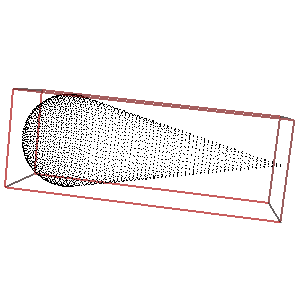
\includegraphics[scale=0.4]{./img/geometric_01}
  \caption{Illustration of the geometric clustering on a cone-sphere.}
     \end{center}
     \end{figure}
}
\only<3|handout:5>{
\begin{figure}[H]
    \begin{center}
  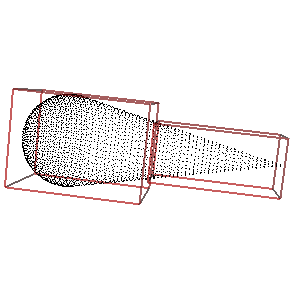
\includegraphics[scale=0.4]{./img/geometric_02}
  \caption{Illustration of the geometric clustering on a cone-sphere.}
     \end{center}
     \end{figure}
}
\only<4|handout:5>{
\begin{figure}[H]
    \begin{center}
  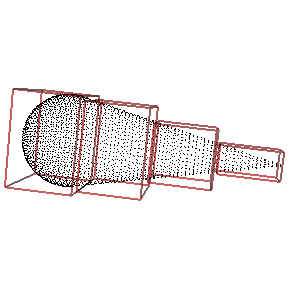
\includegraphics[scale=0.4]{./img/geometric_03}
  \caption{Illustration of the geometric clustering on a cone-sphere.}
     \end{center}
     \end{figure}
}
\only<5|handout:5>{
\begin{figure}[H]
    \begin{center}
  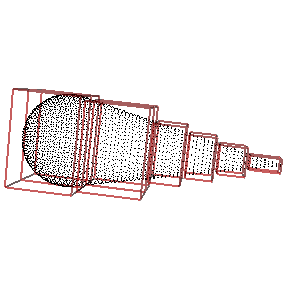
\includegraphics[scale=0.4]{./img/geometric_04}
  \caption{Illustration of the geometric clustering on a cone-sphere.}
     \end{center}
     \end{figure}
}
\end{frame}
